\documentclass[Interploate_hadwritten_Digits.tex]{subfiles}

\begin{document}
	\subsection{Erkennen von Ziffern}
	\label{sec:results_classification}
	Das Neuronale Netz zum Erkennen der Ziffern erreicht nach 100 Trainingsiterationen im Normalfall eine Genauigkeit von circa 88\%, wie in der Abbildung \ref{fig:hist_network_accuracy} zu erkennen ist. Es gibt einige Ausreisser, welche schlechtere Werte haben, die sind aber die Ausnahme. Auch lassen sich in den Konfusionsmatrizen keine grossen Fehler erkennen. Erhöhte Fehlerwerte lassen sich lediglich bei ähnlichen Ziffern (wie 3 \& 5 oder 4 \& 9) erkennen. Alle Konfusionsmatrizen sind im Anhang im Kapitel \ref{sec:apendix_konfusion_network} zu finden.
	\begin{Figure}
		\centering
		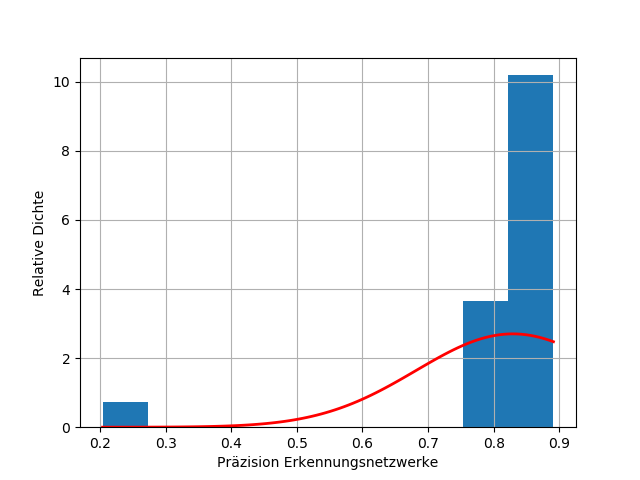
\includegraphics[width=\linewidth]{img/results/histogram_network_accuracy.png}
		\captionof{figure}{Präzision des Neuronalen Neztes}
		\label{fig:hist_network_accuracy}
	\end{Figure}

	\subsection{Netzwerk Komprimierung}
	\label{sec:results_compression}
	Die Komprimierung des Netzwerkes gemäss Kapitel \ref{sec:method_compress} in eine Matrix führt zu einem starken Qualitätsverlust der Vorhersagen. Der grosse Teil der komprimierten Netze erreicht eine Trefferquote von 30\%, wie in Abbildung \ref{fig:hist_compressed_network_accuracy} zu erkennen ist. Dies sind die Resultate der Neuronalen Netze aus dem Kapitel \ref{sec:results_classification}. Es sind Ausreisser zu erkennen, deren Werte liegen aber mit einer Trefferquote von maximal 45\% weit entfernt von den Werten der unkomprimierten Netze.
	\begin{Figure}
		\centering
		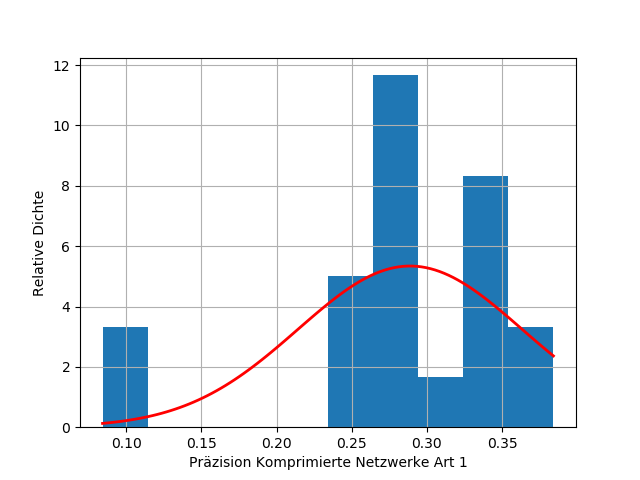
\includegraphics[width=\linewidth]{img/results/histogram_compressed_network_accuracy.png}
		\captionof{figure}{Präzision des komprimierten Neuronalen Neztes Methode 1}
		\label{fig:hist_compressed_network_accuracy}
	\end{Figure}

	In der zweiten Methode der Komprimierung, bei welcher die Aktivierungsfunktion nur auf das Resultat der Vorhersage anwendet, ist ebenfalls eine Verschlechterung der Werte zu erkennen. Diese ist sogar noch stärker. So verteilen sich die Werte gemäss Abbildung \ref{fig:hist_compressed_network_v2_accuracy} zwischen 10\% und 20\%. Es gilt zu beachten, dass die Verteilung der Resultate durch die Untergrenze von 10\% begrenzt ist. Dieser Wert ist für eine zufällige Klassifizierung zu erwarten. Somit bietet der grösste Teil der Netze, welche auf diese Art komprimiert wurden, keinen Mehrwert.
	\begin{Figure}
		\centering
		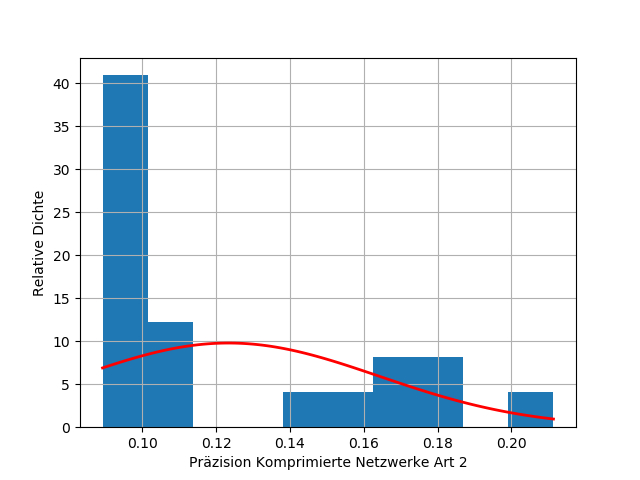
\includegraphics[width=\linewidth]{img/results/histogram_compressed_network_v2_accuracy.png}
		\captionof{figure}{Präzision des komprimierten Neuronalen Neztes Methode 2}
		\label{fig:hist_compressed_network_v2_accuracy}
	\end{Figure}

	Die Invertierung mit mehreren Matrizen erreicht die selben Werte wie die unkomprimierten Versionen. Dies ist in der Abbildung \ref{fig:hist_inverted_network_accuracy} zu erkennen. Aus diesem Grund wurde diese Art der Komprimierung für das Generieren der Bilder im weiteren Verlauf der Arbeit verwendet.
	\begin{Figure}
		\centering
		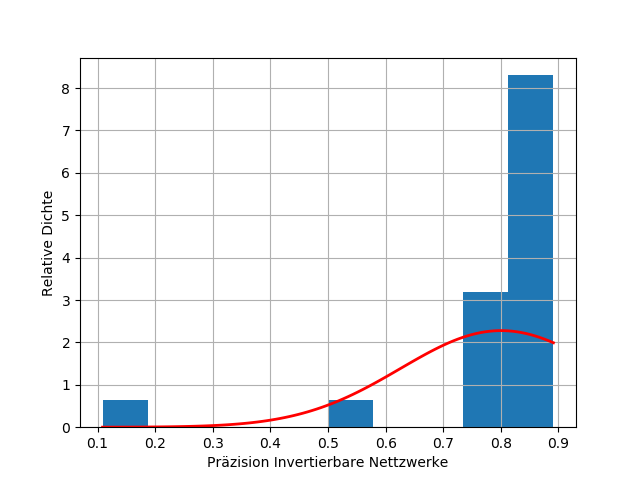
\includegraphics[width=\linewidth]{img/results/histogram_inverted_network_accuracy.png}
		\captionof{figure}{Präzision des komprimierten Neuronalen Neztes mehrere Matrizen}
		\label{fig:hist_inverted_network_accuracy}
	\end{Figure}
	
	\subsection{Invertierung mit Pseudoinvers}
	Auf den Bildern, welche durch die Invertierung des Neuronalen Netzes mit Hilfe des Pseudoinversen entstanden, ist nur Rauschen zu erkennen. In der Abbildung \ref{fig:dig_ideal_0_inverted} ist das errechnete Bild für den Vektor $ \begin{bmatrix}1 & 0 & 0 & 0 & 0 & 0 & 0 & 0 & 0 & 0 \end{bmatrix}^{T} $ zu sehen. Dies würde einer idealen Null entsprechen. Auf den Resultaten von anderen Ziffern lassen sich ebenfalls keine Ziffern erkennen. Auch sind von Auge keine Muster zwischen den Bildern zu erkennen. Weitere Bilder zum Vergleich sind im Anhang im Kapitel \ref{sec:apendix_numbers_inversion} zu finden.
	\begin{Figure}
		\centering
		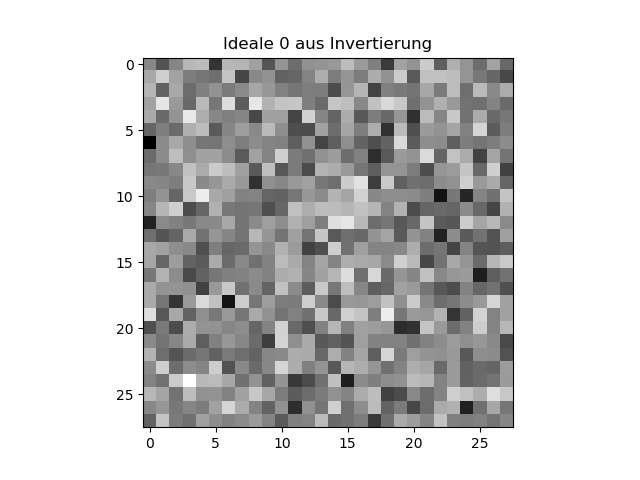
\includegraphics[width=\linewidth]{img/results/ideal_0_inverted.png}
		\captionof{figure}{Ideale 0 aus Invertierung}
		\label{fig:dig_ideal_0_inverted}
	\end{Figure}

	Ähnliche Resultate sind auch bei den interpolierten Ziffern zu sehen. In der Abbildung \ref{fig:dig_interpolated_4_9_50_inverted} ist eine Interpolation zwischen einer idealen Vier und einer idealen Neun abgebildet. Der Winkel für die Interpolation wurde so gewählt, dass sich der Vektor genau zwischen den beiden Werten befindet. Wie bereits bei den idealen Ziffervektoren lassen sich im Bild keine Ähnlichkeiten mit den im Eingabevektor definieren Ziffern erkennen.
	\begin{Figure}
		\centering
		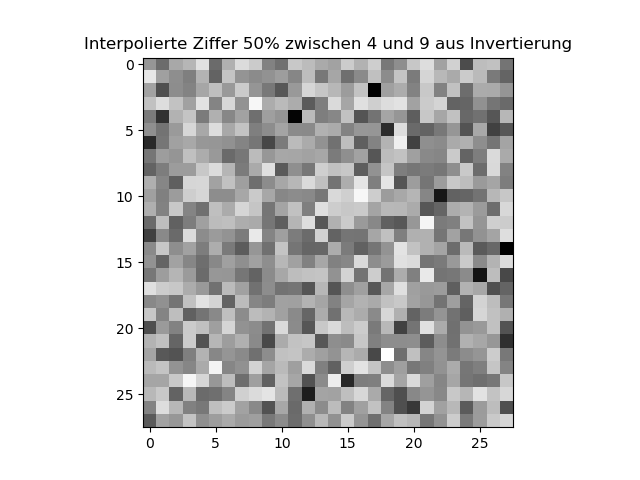
\includegraphics[width=\linewidth]{img/results/interpolated_4_9_50_inverted.png}
		\captionof{figure}{Interpolation von 4 und 9 durch Invertierung}
		\label{fig:dig_interpolated_4_9_50_inverted}
	\end{Figure}
	
	\subsection{Invertierung mit quadratischen Matrizen}
	Das Trainieren eines Neuronalen Netzes, welches nur quadratische Matrizen verwendet, erwies sich als äussert schwierig. Die Trainingszeiten wuchsen stark an und die Resultate waren deutlich schlechter als die der Netze ohne quadratischen Matrizen. Der Abbildung \ref{fig:hist_squared_network_accuracy} kann entnommen werden, dass die meisten Netzwerke mit quadratischen Matrizen Trefferquoten von ungefähr 12\% bis 16\% erreichen. Es gilt auch festzuhalten, dass ein grosser Teil der trainierten Netze lediglich 10\% der Bilder korrekt klassifiziert, was einer zufälligen Klassifikation entspricht.
	\begin{Figure}
		\centering
		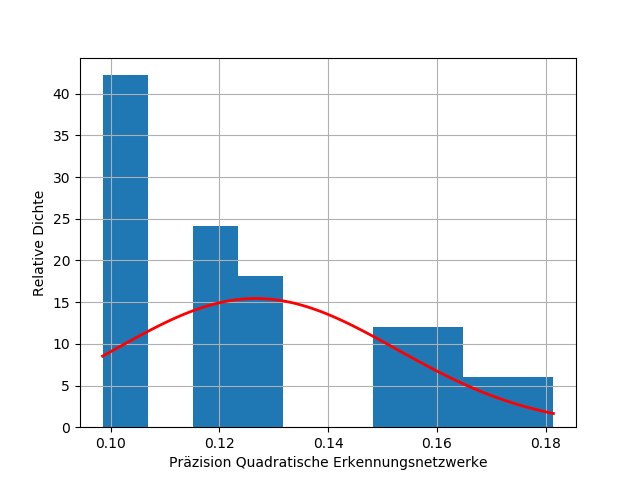
\includegraphics[width=\linewidth]{img/results/histogram_squared_network_accuracy.png}
		\captionof{figure}{Präzision des Neuronalen Neztes mit quadratischen Matrizen}
		\label{fig:hist_squared_network_accuracy}
	\end{Figure}

	Wegen der Schwierigkeit Neuronale Netze mit quadratischen Matrizen zu trainieren, musste bestimmt werden, ob dieser Ansatz für diesen Bericht weiterverfolgt wird. Daher wurde Untersucht, ob eine Invertierung eines Neuronalen Netzes mit ausschliesslich quadratischen Matrizen realisierbar ist.  Die Resultate dazu sind im Kapitel \ref{sec:results_error_inverse} zu finden.
	
	\subsection{Fehler bei Gleitkommazahloperationen}
	\label{sec:results_error_inverse}
	Um zu bestimmen, wie sich die Rundungsfehler der Gleitkommazahlen auf Invertierung des Neuronalen Netzwerks auswirken, wurden verschiedene zufällig generierte Matrizen vor- und rückwärts durch das Neuronalen Netz gerechnet und der durchschnittliche Fehler pro Wert in der Matrix bestimmt. Die Matrizen wurden so gewählt, dass $ M \in \mathbb{R}^{n \times n}, n \in [3, 9] $ und im Neuronalen Netz aus einer bis vier Schichten besteht. Die Resultate sind der Tabelle \ref{tbl:reverse_error} zu entnehmen.Daraus lässt sich erkennen, dass bei einer Matrix aus $ \mathbb{R}^{9 \times 9} $ bereits ein Netzwerk mit einer Schicht die Werte nach der Invertierung im Schnitt im Bereich von $ 10^{0} $ verändert. Bei vier Schichten wird dieser Wert bereits bei einer Matrix aus $ \mathbb{R}^{6 \times 6} $ überschritten.
	\begin{table}[H]
		\centering
		\begin{tabular}{|l|r|r|r|r|}
			\hline
			 & 1 Layer & 2 Layers & 3 Layers & 4 Layers  \\ \hline
			$ \mathbb{R}^{3 \times 3} $ & 8.2e-15 & 3.8e-12 & 1.5e-08 & 1.6e-09 \\ \hline
			$ \mathbb{R}^{4 \times 4} $ & 1.6e-13 & 3.3e-10 & 3.35e-05 & 1.7e-04 \\ \hline
			$ \mathbb{R}^{5 \times 5} $ & 1.9e-10 & 5.0e-08 & 2.3e-06 & 6.1e-03 \\ \hline
			$ \mathbb{R}^{6 \times 6} $ & 1.0e-02 & 1.6e-02 & 3.4e-02 & 4.7e+00 \\ \hline
			$ \mathbb{R}^{7 \times 7} $ & 9.7e-02 & 2.3e-01 & 2.5e+00 & 1.3e+01 \\ \hline
			$ \mathbb{R}^{8 \times 8} $ & 4.5e-01 & 2.3e-01 & 6.2e+00 & 1.7e+01 \\ \hline
			$ \mathbb{R}^{9 \times 9} $ & 2.1e+00 & 1.6e+00 & 7.3e+00 & 1.9e+01 \\ \hline
		\end{tabular}
		\caption{Durchschnittlicher Fehler pro Wert nach Invertierung}
		\label{tbl:reverse_error}
	\end{table}	
	
	\subsection{Approximieren der Inputbilder}
	\label{sec:results_appriximation}
	Wegen der signifikanten Fehler aus der Rundung der Gleitkommazahlen im Ansatz der Invertierung wurde der Ansatz der Approximation von Bildern weiterverfolgt. Bei diesem Ansatz wurde als Qualitätsmass der Fehler aus der Kreuzentropie zwischen dem erreichten Vektor und dem gewünschten Vektor für das zu generieren Bild verwendet. Hier lassen sich deutliche Unterschiede für die Approximation der idealen Ziffern und der interpolierten Ziffern erkennen. In der Abbildung \ref{fig:hist_approximation_error_ideal} ist zu erkennen, dass für die idealen Ziffern der durchschnittliche Fehler bei 1.5 liegt, wobei es auch einige Ausreisser bei über 2.2 gibt.
	\begin{Figure}
		\centering
		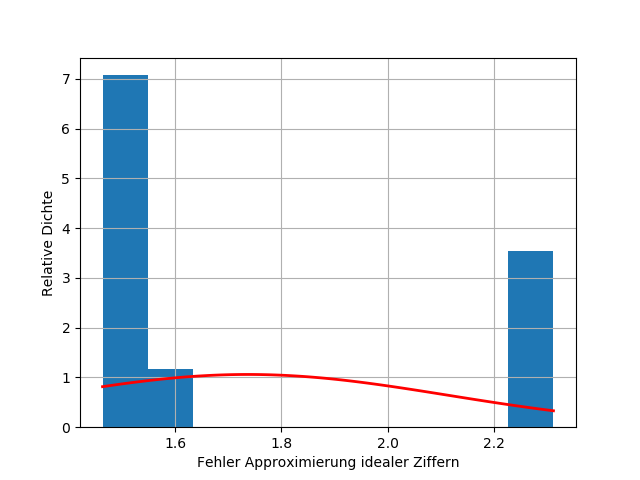
\includegraphics[width=\linewidth]{img/results/histogram_approximation_error_ideal.png}
		\captionof{figure}{Fehler bei Approximation idealer Ziffern}
		\label{fig:hist_approximation_error_ideal}
	\end{Figure}	
	
	In der Abbildung \ref{fig:hist_approximation_error_interpolation} ist zu erkennen, dass der Fehler der interpolierten Ziffern höher liegt als der der idealen Ziffern. Ebenfalls lässt sich erkennen, dass der Median in der Nähe von 2.2 liegt, was an den Fehlerwert der Ausreisser bei den idealen Ziffern erinnert.
	\begin{Figure}
		\centering
		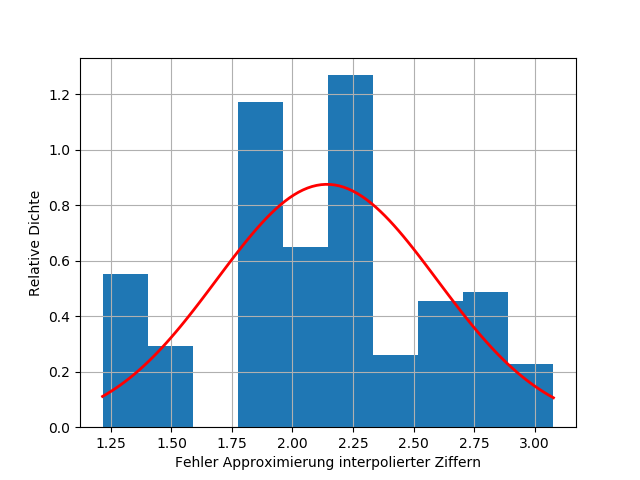
\includegraphics[width=\linewidth]{img/results/histogram_approximation_error_interpolation.png}
		\captionof{figure}{Fehler bei Approximation interpolierter Ziffern}
		\label{fig:hist_approximation_error_interpolation}
	\end{Figure}
	
	Die generierten Bilder enthalten auch hier nur Rauschen. Auch bei den tiefen Fehlerwerten der idealen Ziffern ist keine Struktur zu erkennen. In der Abbildung \ref{fig:dig_ideal_7_approximated} ist das approximierte Bild für eine ideale 7 zu sehen.
	\begin{Figure}
		\centering
		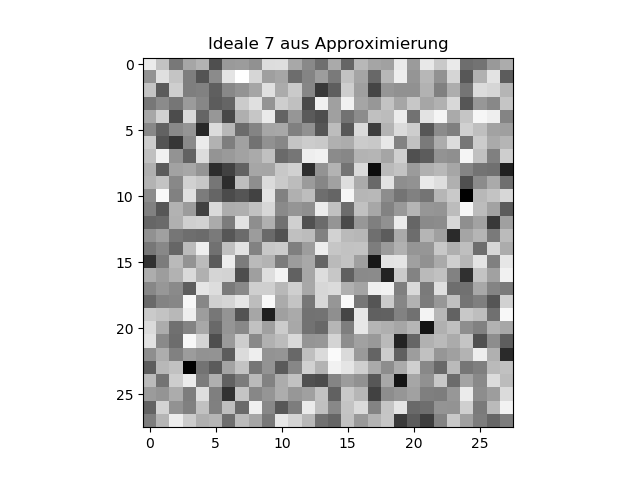
\includegraphics[width=\linewidth]{img/results/ideal_7_approximated.png}
		\captionof{figure}{Ideale 7 durch Approximierung}
		\label{fig:dig_ideal_7_approximated}
	\end{Figure}
	
	In einem letzten Versuch wurden für die Approximation anstelle von zufällig generierten Matrizen als Startpunkt Bilder aus dem Trainingssatz verwendet. Dies führte dazu, dass die Approximation die Inputmatrix nicht veränderte, auch wenn eine andere Ziffer als Ziel der Approximation angegeben wurde.

\end{document}